\documentclass[a4paper]{jpconf}
\usepackage{graphicx}
\usepackage{amsmath,amsfonts,amssymb,amsthm,siunitx,bm}
\numberwithin{equation}{section}
\newtheorem*{note}{Note}

\begin{document}
\title{Electron spin resonance and nuclear magnetic resonance}
\author{2197055}

\begin{abstract}
Electron spin resonance (ESR) and nuclear magnetic resonance (NMR) are two important spectroscopic techniques for probing properties of materials containing constituents with non-zero permanent magnetic moments capable of resonant absorption of electromagnetic energy --- electronic systems in the case of ESR and atomic nuclei in the case of NMR. In this experiment, we studied ESR on a sample of Diphenyl-Picryl-Hydrazil (DPPH), a paramagnetic organic molecule with an unpaired $e^-$, by means of measuring the resonant frequency as a function of externally applied magnetic field, in order to determine the sample\textquoteright s $g$-factor, which was found to be $g\textsubscript{DPPH} = 2.02 \pm 0.01$.
Further, we investigated the magnetic properties of ${}^1$H and ${}^{19}$F nuclei in the following substances: glycerine, polystyrene (both of which contain hydrogen), PTFE (which contains fluorine), and polythene, whose composition we wanted to learn about. The experimentally measured $g$-factors were $g\textsubscript{glycerine} = 5.54 \pm 0.03$, $g\textsubscript{polystyrene} = 5.68 \pm 0.01$ and $g\textsubscript{PTFE} = 5.34 \pm 0.01$. Comparison with the results obtained for polythene lead us to postulate the presence of hydrogen in our polythene sample, as confirmed by its chemical formula.
\end{abstract}

\section{Introduction}
Electron spin resonance (ESR), also referred to as electron paramagnetic resonance (EPR) spectroscopy,      % find reference
is an important method for studying paramagnetic chemical substances, in which the electrons' magnetic moments don't cancel, such as organic and inorganic free radicals or transition-metal ion complexes. It can provide detailed information relating to the chemical composition and structure of materials, and therefore finds innumerable applications in biology, chemistry, materials science, medicine and pharmacology, to name just a few.

Similarly, nuclear magnetic resonance (NMR) exploits the fact that some nuclei possess a non-zero overall spin, and hence a permanent magnetic moment, to probe the properties of materials containing such nuclei. It has widespread use and far-reaching applications, notably in medical imaging, where it forms the basis behind MRI (magnetic resonance imaging).

The aim of this experiment was to explore the fundamental principles underlying these two phenomena.

\section{ESR}
In the first part of the experiment, we performed an ESR study on a sample of Diphenyl-Picryl-Hydrazil (DPPH), which is a paramagnetic organic molecule with a single unpaired $e^-$. The orbital angular momentum of this electron is essentially zero,    % find reference
and hence the molecule\textquoteright s total magnetic moment is solely due to the electron\textquoteright s intrinsic spin angular momentum, which makes it particularly suited for ESR investigations.
 
\subsection{Theory}\label{section: theory}
In the absence of any external magnetic fields (i.e.\ for a free $e^-$), the two possible spin states (``spin up'' and ``spin down'') are degenerate --- they have the same energy.

However, \emph{energy splitting} occurs when the electron is placed in a magnetic field. Indeed, the intrinsic spin gives rise to a magnetic moment $\bm{\mu}_S$ which interacts with the applied field and possesses a different energy depending on its relative spatial orientation. 

According to quantum mechanics, only two configurations are possible. The magnitude $S$ of the spin vector $\mathbf{S}$, and its two allowed $z$-components $S_z$ (where the $z$-axis is defined to lie along the direction of the field), are respectively given by
\begin{align}
	S &= \lvert\lvert\mathbf{S}\rvert\rvert = \sqrt{s(s+1)}\hbar = \tfrac{\sqrt{3}}{2}\hbar,  \quad \text{and} \nonumber \\
	S_z &= m_s \hbar. \label{eqn: magnetic moment z-projection}
\end{align}
where $s=\tfrac12$ is the spin quantum number, $m_s=\pm\tfrac12$ is the secondary spin quantum number, and $\hbar = \tfrac{h}{2 \pi}$ is the reduced Planck\textquoteright s constant.

The associated magnetic moment is
\begin{align}
	\bm{\mu}_S = - g \frac{\mu_B}{\hbar} \mathbf{S} \label{eqn: magnetic moment}
\end{align}
where $g$ is the Land\'e splitting factor, or $g$-factor (which for a free electron has the value $g_e = 2.002319$), and $\mu_B = 9.274 \times 10^{-24} \si{\joule\per\tesla}$ is the Bohr magneton. 

A magnetic moment $\bm{\mu}_S$ in a field $\mathbf{B} = B \, \mathbf{e_z}$ (where $\mathbf{e_z}$ is the unit vector in the $z$-direction) has potential energy
\begin{equation}
	E = - \bm{\mu}_S \cdot \mathbf{B} \underset{\text{\eqref{eqn: magnetic moment}}}{=}  - (- g \frac{\mu_B}{\hbar} \mathbf{S})\cdot\mathbf{B}
	  \underset{\text{\eqref{eqn: magnetic moment z-projection}}}{=} g \frac{\mu_B}{\hbar}S_z B 
	  = g\mu_Bm_sB \label{eqn: potential energy}.
\end{equation}

Equation \eqref{eqn: potential energy} shows that the two orientations ($m_s = \pm\tfrac12$) no longer have the same energy --- the one whose magnetic moment is aligned with the field (or equivalently whose spin points in the direction opposite to the field, i.e.\ $m_s = -\tfrac12$) has a lower potential energy than the one whose magnetic moment is anti-parallel to the field, as depicted in figure \ref{fig: energy splitting}. The energy difference between the two levels is 
\begin{equation}
	\Delta E = g \mu_B B. \label{eqn: energy difference}
\end{equation}

\begin{figure}[htbp]
	\includegraphics[scale=0.75]{EPR_splitting.png}
	\hspace{2pc}
	\begin{minipage}[b]{3in}
		\caption{Energy splitting of the two spin states of an $e^-$ placed in an external magnetic~field~$\mathbf{B_0}$.}
	\end{minipage}
	\label{fig: energy splitting}
\end{figure}

In thermal equilibrium, the spins are distributed according to the Boltzmann distribution
\[
    \frac{N_{+\tfrac12}}{N_{-\tfrac12}} = \exp(- \frac{\Delta E}{k_B T}),
\]
where $k_B$ is Boltzmann\textquoteright s constant, and $N_{\pm\tfrac12}$ are the number of spins in the higher and lower states, respectively. 

If there is a predominance of spins in the lower state, transitions can be induced by supplying energy to the sample, for instance by irradiating it with electromagnetic (EM) radiation of the right frequency $\nu$. The energy of an EM wave is $h \nu$, where $h$ is Planck's constant, so the condition for resonance, using \eqref{eqn: energy difference}, can be stated as
\begin{equation}
	h\nu = g\mu_B B. \label{eqn: resonance condition}
\end{equation}

In a real material, an electron ``feels'' also fields produced by any surrounding magnetic nuclei and/or other electrons, whose effect can be interpreted in terms of a shift in the $g$-factor compared to the free-electron value, and in this particular experiment, we were measuring the $g$-value of DPPH. In addition, the chemical environment also has an effect on the shape of the resonance signal and its line width, amongst other things, which gives an indication of how ESR can be used to infer information about the chemical composition and structure of materials. 

\subsection{Experimental method}\label{section: method}
% Insert figure
The DPPH sample was placed in a uniform magnetic field generated by two parallel vertical Helmholtz coils (HCs) connected to a DC current supply. The sample was inserted into another coil connected to an RF circuit oscillating at an adjustable frequency $\nu$, irradiating the sample with energy $h\nu$. The magnetic field produced by the HCs was varied by changing the current, and resonance was detected with an oscilloscope thanks to an observable voltage change in the RF circuit that occurred each time the condition \eqref{eqn: resonance condition} was met for a particular (fixed) frequency. The measurement was repeated for a number of different frequencies.  

For an $e^-$ with only two possible spin states, it would be necessary to match the RF frequency and the current in the HCs with considerable accuracy to obtain resonance. Also, once the population of the spin states has been inverted, the sample can no longer absorb more energy before enough electrons have returned to the lower state, so they need to be excited at a rate slower than the relaxation time (the time needed for the electrons to de-excite and return to thermal equilibrium via spin-spin and spin-lattice interactions). 

A solution to both issues was to superimpose a ($50 \si{\hertz}$) modulation (AC) current on the DC component going into the HCs, resulting in a sinusoidally-varying modulation magnetic field. The total field $\mathbf{B}_{total}$ was then the superposition of the two, and thus oscillated around a central value $B_0$. If the resonance condition \eqref{eqn: resonance condition} was satisfied for some value of $\mathbf{B}_{total}$ during this oscillation, a resonance signal was observed, twice during the cycle at symmetric positions (provided that the phase lag between the modulation signal and the sample response signal was correctly accounted for). By adjusting the DC current, it was possibly to make the resonance occur precisely at the point when the modulation field dropped to zero and the field was equal simply to $B_0$, i.e.\ it was the $B_0$ that satisfying \eqref{eqn: resonance condition} for the given frequency.

The value of $B_0$ could be deduced from the DC current $I_0$ in the coils --- we created a calibration curve of $B_0$ as a function of $I_0$ using a Hall probe sensor to measure the magnetic field in the centre of the coil set-up.

\subsection{Results}
The results of the two stages of the experiment are summarized in the following subsections.

\subsubsection{Helmholtz coils calibration.} \label{section: calibration}
The direct current going through the Hemlhotz coils was varied and the magnetic field $B_0$ at the centre of the coils was recorded. We observed quite large fluctuations of the field for a given current, and therefore 5 different readings were taken and averaged. For the purposes of error analysis, the uncertainty in the mean was then taken to be half the spread of the observed values (as there weren't enough readings to justify using the formula for the standard error in the mean). For the current, the measurement uncertainty was taken to be half the smallest scale division. 

We subsequently performed a weighted straight-line fit to the data. Figure \ref{fig: HC calibration curve} shows the resulting calibration curve with uncertainties indicated by error bars. This curve was used in the second part to convert between measured current and magnetic field applied to the sample. We used the MATLAB's built-in function \texttt{polyval} to estimate the uncertainties in the values of $B_0$ predicted by the curve, based on the goodness of fit.

We obtained 
\[
	B_0 = (3.73 \pm 0.01) I + (0.03 \pm 0.01),
\]
where $I$ is in $\si{\ampere}$, and $B_0$ is in $\si{\milli\tesla}$.

\subsubsection{Measurement of the $g$-factor of DPPH.}
The frequency in the RF oscillator circuit was varied in steps of $5 \si{\mega\hertz}$, and for each frequency, the current in the Helmholtz coils was scanned over the range $0.1 \si{\ampere}$ to $1.2 \si{\ampere}$ to find the resonance. For a given frequency, the measurement was repeated multiple times to get an idea of the uncertainty in the resonant current. Figure \ref{fig: DPPH resonance} shows the resonance frequency as a function of the field.

\begin{figure}[htbp]
	\begin{minipage}[b]{2.9in}
		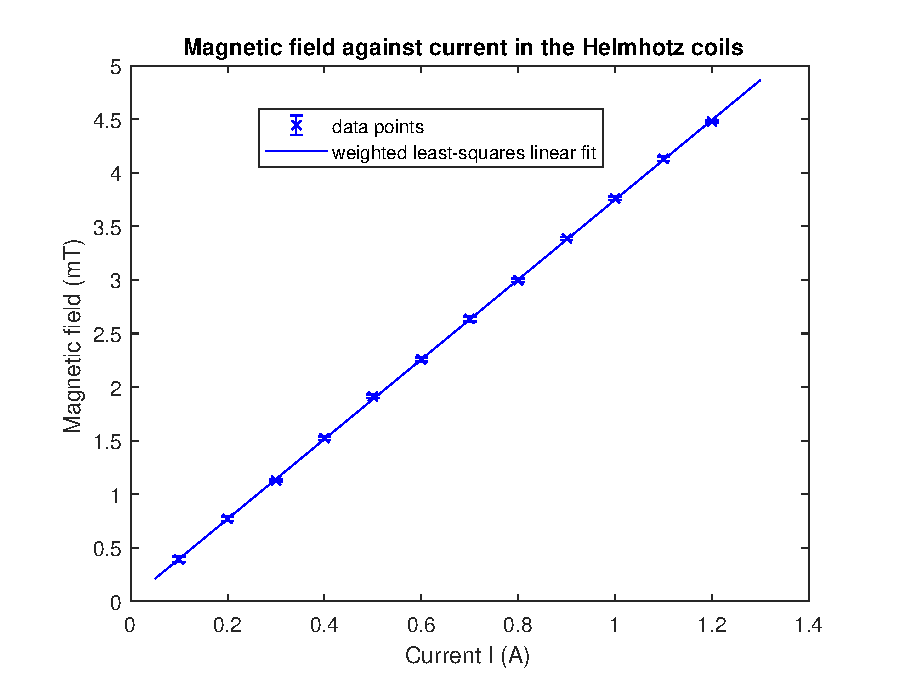
\includegraphics[scale=0.59]{ESR_calibration.eps}
		\caption{Magnetic field in between the Helmholtz coils as a function of the current passing through them.}
		\label{fig: HC calibration curve}
	\end{minipage}
    \hspace{1.5pc}
	\begin{minipage}[b]{3in}
		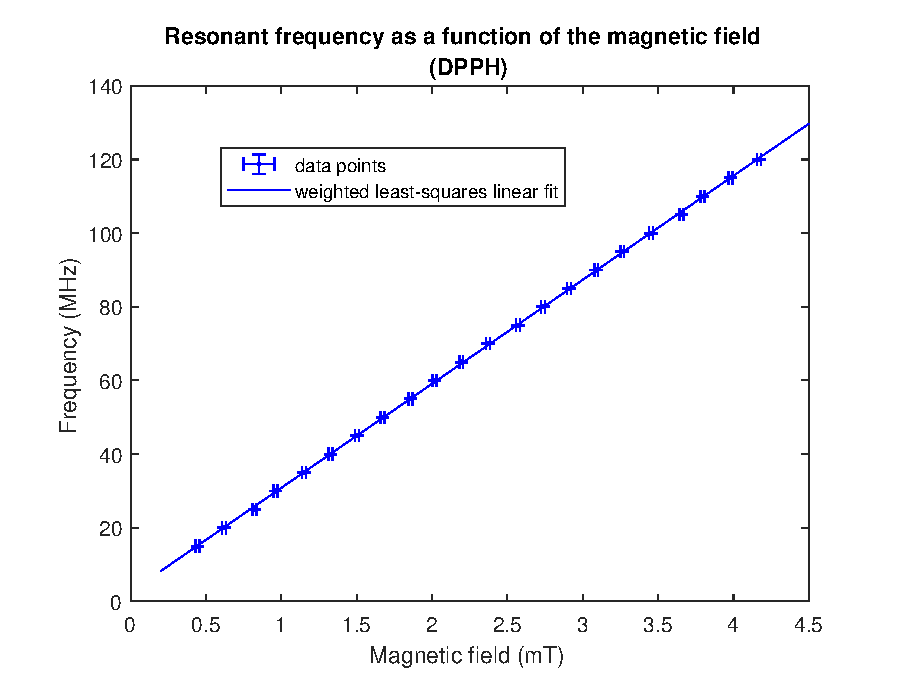
\includegraphics[scale=0.6]{DPPH.eps}
		\caption{Resonant frequency as a function of applied magnetic field for the DPPH sample.}
		\label{fig: DPPH resonance}
	\end{minipage}
\end{figure}

\subsection{Analysis}
According to equation \eqref{eqn: resonance condition}, the plot of frequency $\nu$ against magnetic field $B_0$ should be a straight line with gradient 
\[
	\frac{\nu}{B_0} = \frac{g_{\textsubscript{DPPH}} \mu_B}{h},
\]
which implies
\begin{equation} \label{eqn: gradient}
	g_{\textsubscript{DPPH}} = \left(\frac{h}{\mu_B}\right) \left(\frac{\nu}{B_0}\right). 
\end{equation}
	
From the weighted straight-line fit to our data shown in figure \ref{fig: DPPH resonance}, we have
\[
	\left(\frac{\nu}{B_0}\right) = 28.24 \pm 0.07 \; \si{\mega\hertz\per\milli\tesla}.
\]

Substituting into \eqref{eqn: gradient} yields 
\[
	g_{\textsubscript{DPPH}} = 2.02 \pm 0.01,
\] 
(where the uncertainty in the final value has been computed, given that $h$ and $\mu_B$ are constants, simply by multiplying the error in the gradient by $h / \mu_B$ ).

\subsection{Discussion}
For a pair of Helmholtz coils separated by a distance equal to their radius, the theory of electromagnetism predicts that the value of the field at the centre should obey approximately
\[
	B_0 = \mu_0 \left(\frac45\right)^{\tfrac32} \frac{n}{r} I,
\]
where $\mu = 4\pi\times10^{-7} \; \si{\volt\s\ampere\tothe{-1}\meter\tothe{-1}}$, $n$ is the number of turns per coil, and $r$ is their radius.

This shows that the expected relationship between $I$ and $B_0$ is linear, as confirmed by our data (see figure \ref{fig: HC calibration curve}).
However, for our particular coils, the expected value of the gradient was $4.23$, which does not agree with the one we obtained experimentally, i.e.\ $3.73 \pm 0.01$. This could be due to the fact that the separation of the coils might not have been exactly equal to their radius. Due to such possible differences in our set-up from the idealised case, we used the experimentally obtained calibration curve in subsequent calculations, not the theoretical one. Any error in the calibration curve therefore represents a systematic error in the results obtained thereafter.

Possible sources of error were the difficulty in making sure that the Hall probe was oriented perpendicularly to the measured field (i.e.\ parallel to the coils), and that it was located at the exact position where the sample was later placed. We also couldn't be sure whether the Hall probe itself was calibrated correctly (as we didn't obtain the expected result when we checked with a standard magnet), and whether we zeroed it at a point with no magnetic field. This could have introduced a systematic offset. A source of statistical errors were the random fluctuations in the magnetic field as well as in the response of the probe over time (e.g.\ due to warming up of the equipment or other reasons).

The accepted value for the $g$-factor of DPPH is
\[
	g_{\textsubscript{DPPH, th}} = 2.0036.
\]
Our value lies within $2\sigma$ of this value, and is therefore in reasonable agreement.
Compare this with the theoretical value for the spin $g$-factor of a free $e^-$, which is
\[
	g_{e,\text{ th}} = 2.002319.
\]
This is slightly different from both the accepted and our experimental value for $g_{\textsubscript{DPPH}}$, which, as explained in the section \ref{section: theory}, could stem from the effect of the chemical surrounding of the unpaired $e^-$. Nevertheless, the values are relatively close, showing in particular that the assumption that we can neglect the orbital angular momentum of the $e^-$, and attribute the molecule's magnetic moment solely to the intrinsic spin is largely justified.


\section{NMR} 
In the second part of the experiment, we performed NMR on protons and fluorine atoms in both liquid and solid samples, namely in glycerine and polystyrene (which contain ${}^1$H), PTFE (containing ${}^{19}F$), and polythene, about which we wanted to determine whether it is more likely to contain hydrogen or fluorine.
\subsection{Theory}

The basic principles of NMR are essentially the same as those of ESR. Atomic nuclei that have an odd number of nucleons can have a non-zero overall nuclear spin $\mathbf{S}$ which gives rise to a nuclear magnetic moment $\bm{\mu}_n$. When placed in a magnetic field, either external, or due to other close-by magnetic nuclei or the orbiting electrons, the nuclear spin can adopt, quantum-mechanically speaking, $2S + 1$ possible orientations, each corresponding to a different energy level
\[
	E_n = -g \mu_n B_0 n, \quad n = -S, -S+1, \dots, 0, \dots, S. 
\] 
The $g$-factor again depends on the chemical environment and bond structure (so-called ``chemical shift''). 

All of our samples had $S = \tfrac{1}{2}$, which meant there were only two possible spin levels, and the condition for resonance was 
\begin{equation}\label{eqn: NMR resonance condition}
	h\nu = \Delta E = -g \mu_n B_0.
\end{equation}


\subsection{Experimental method}
The experimental procedure was analogous to the ESR part of the experiment (see section (\ref{section: method})). The only differences were that the static magnetic field was generated by an iron-cored electromagnet, instead of Helmholtz coils, and the modulating field was produced by a pair of smaller attached modulation coils.


\subsection{Results}
\subsubsection{Electromagnet calibration.}
Just like in section \ref{section: calibration}, we first calibrated the electromagnet to be able to relate the current passing through it to the magnetic field it generates. Since the electromagnet contained an iron core, its field depended not only the value of the current, but also on whether the current was being increased or decreased. This effect is called \emph{hysteresis} (a dependence of the net magnetization of a ferromagnet on the history of any externally applied magnetic field). 

Therefore, we did our calibration first for an increasing and then a decreasing current. Figure \ref{fig: hysteresis curve} shows the hysteresis curve that we obtained.
\begin{note}
	Only the part of the curve corresponding to increasing current was used in the next section.
\end{note}
We fitted a polynomial of degree $2$, $y = ax^2 + bx + c$, to the upper half of the curve (this was the degree that yielded the lowest error estimates on the fit parameters), with
\begin{align*}
	a &\approx -16 \pm 1, \\
	b &\approx 189 \pm 7, \\
	c &\approx -34 \pm 12.
\end{align*}

%\begin{figure}[htbp]
%	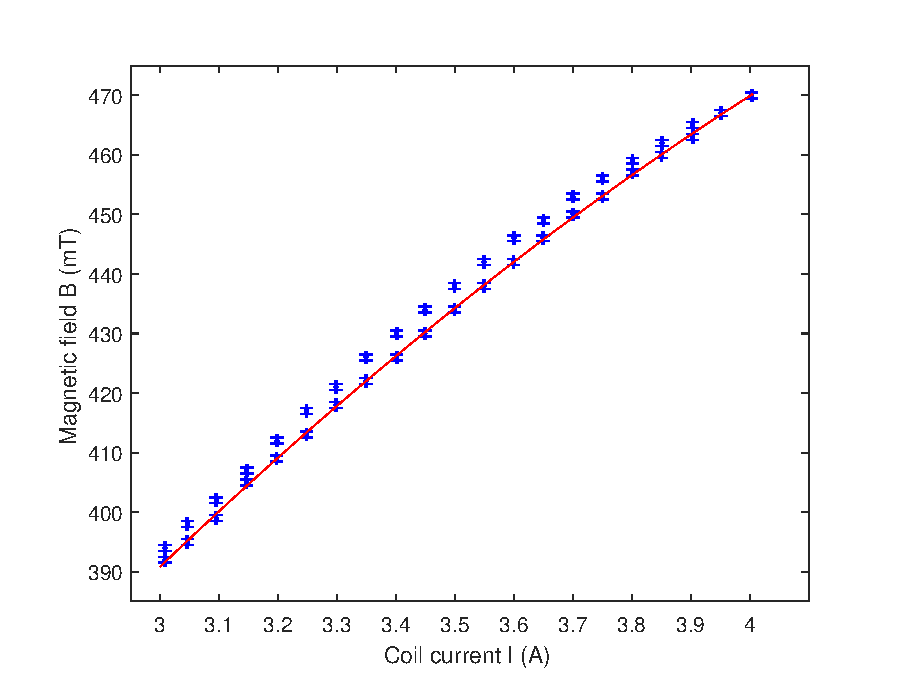
\includegraphics[scale=0.75]{NMR_calibration.eps}
%	\hspace{1pc}
%	\begin{minipage}[b]{2in}
%		\caption{Magnetic field inside the electromagnet as a function of the current.}
%	\end{minipage}
%	\label{fig: hysteresis curve}
%\end{figure}

\subsubsection{Measurement of the $g$-factors of Glycerine, Polystyrene and PTFE.}

Figure \ref{fig: NMR resonances} shows the graphs of resonance frequencies as a function of $B_0$ for the 3 different substances.%, and
%figure \ref{fig: resonance spectra} shows the general shape of the resonance signals as viewed on an oscilloscope.

\begin{figure}[htbp]
	\begin{minipage}[b]{2.9in}
		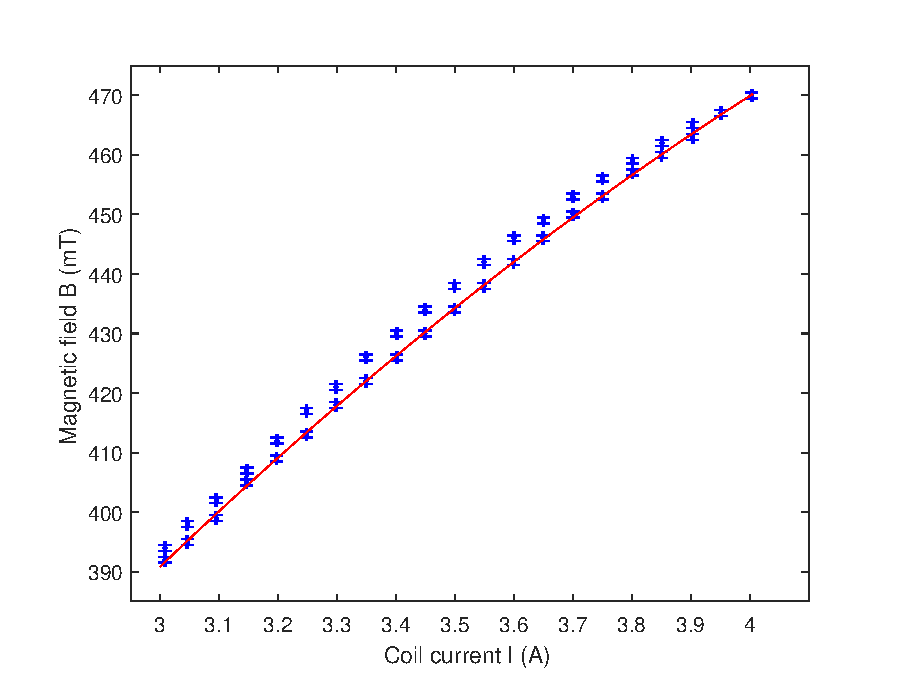
\includegraphics[scale=0.55]{NMR_calibration.eps}
		\caption{Magnetic field inside the electromagnet as a function of the current.}
		\label{fig: hysteresis curve}
	\end{minipage}
	\hspace{1.5pc}
	\begin{minipage}[b]{3.1in}
		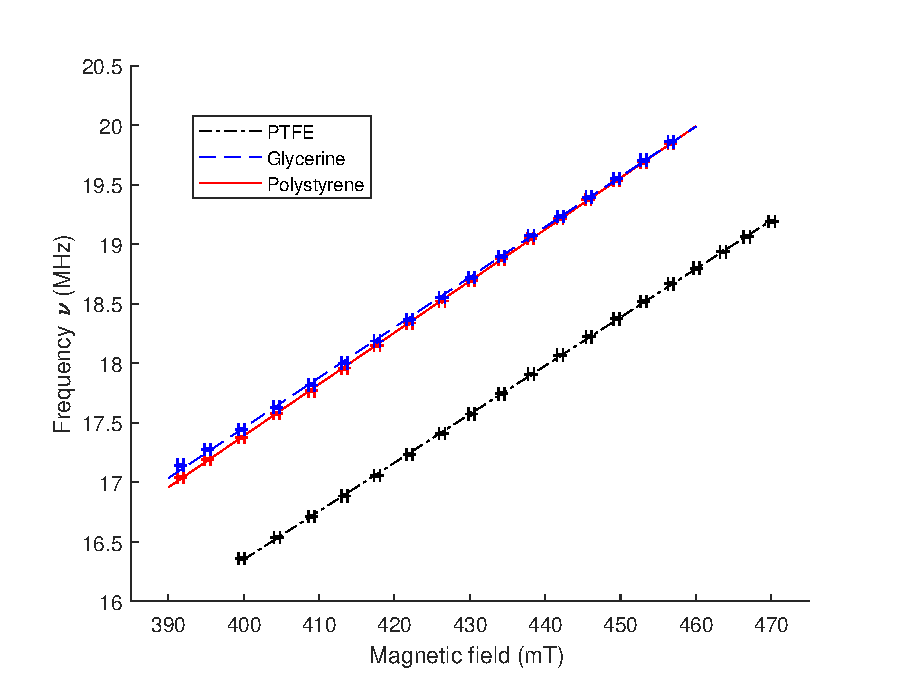
\includegraphics[scale=0.55]{NMR_resonances.eps}
		\caption{Resonant frequency as a function of applied magnetic field for glycerine, polystyrene and PTFE}
		\label{fig: NMR resonances}
	\end{minipage}
\end{figure}

\subsection{Analysis}
According to \eqref{eqn: NMR resonance condition}, $\left| \frac{\nu}{B_0} \right|$ should be a constant, equal to $\frac{g \mu_n}{h}$. It follows that $g = \frac{h}{\mu_n} \left( \frac{\nu}{B_0} \right)$. We performed a straight-line fit to our plots in figure \ref{fig: NMR resonances}, and got
\begin{alignat*}{2}
    &\left( \frac{\nu}{B_0} \right)_{\text{glycerine}} &&= 0.0422 \pm 0.0002 \; \si{\mega\hertz\per\milli\tesla} \\
	&g\textsubscript{glycerine} &&= 5.54 \pm 0.03 \\[12pt]
	&\left( \frac{\nu}{B_0} \right)_{\text{polystyrene}} &&= 0.0433 \pm 0.0001 \; \si{\mega\hertz\per\milli\tesla} \\
	&g\textsubscript{polystyrene} &&= 5.68 \pm 0.01 \\[12pt]
	&\left( \frac{\nu}{B_0} \right)_{\text{PTFE}} &&= 0.0407 \pm 0.0001 \; \si{\mega\hertz\per\milli\tesla} \\
	&g\textsubscript{PTFE} &&= 5.34 \pm 0.01 \\
\end{alignat*}

\subsection{Discussion}

\section{Conclusion}
Our measurements of resonant absorption confirmed the linear relationship predicted by \eqref{eqn: resonance condition} and \eqref{eqn: NMR resonance condition} between the magnetic field and the resonance frequency. They showed that, indeed, in both ESR and NMR, an energy splitting occurs when the sample is placed in an external field, that this creates separate energy levels such that the energy difference between them scales linearly with the applied field, and that energy transitions can be induced by supplying EM energy of the correct frequency. 

An increase in the precision of our findings could have been achieved by taking further repeated measurements, as the statistical errors due to random fluctuations were quite significant, but also by using stronger $\mathbf{B}$ fields, thus increasing the energy differences between the spin states and reducing the relative uncertainty, and/or by operating at lower temperatures, both of which would have potentially resulted in sharper resonance signals with a reduced line width.

\section*{References}
\begin{thebibliography}{9}
\bibitem{iopartnum} 
\end{thebibliography}

\end{document}


